\chapter{Kickstart}

Red Hat Linux提供了一种非常方便的自动化系统安装方式,即为
kickstart\index{kickstart}。这种工具的出现,极大的方便了众多的系统管理
员或装机攻城狮。有了它,我们就不用拿着光盘或U盘在机房来回乱窜地装机了,
我们可以在办公室通过IPMI的方式来操作。不管这个工具有多优秀,相比之前单
台的安装方式,效率提升了很多。当然,也有另外几种较优越的自动化系统安装
工具,这里就不介绍了。

kickstart文件包含了安装程序所使用的指令,在安装的过程中可以用来减少或者
消除用户输入的麻烦。

在系统数目巨大且完全相同的时候,kickstart文件非常有用。


\begin{figure}[htbp]
  \begin{center}
    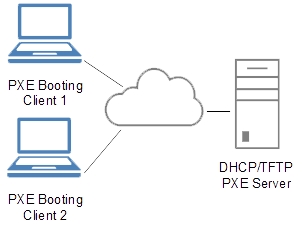
\includegraphics[width=.5\textwidth]{img/PXE_diagram.png}
  \end{center}
  \caption{PXE WorkFlow}
  \label{fig:pxeWork}
\end{figure}

PXE工作流程图:
\begin{figure}[htbp]
  \begin{center}
    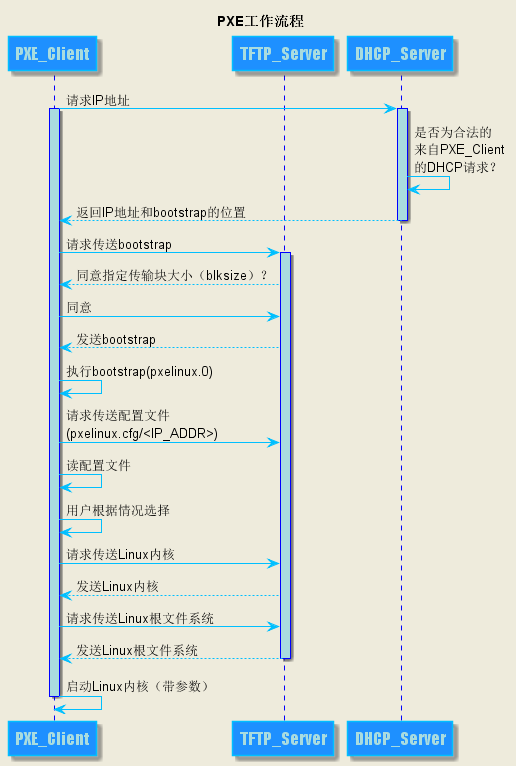
\includegraphics[width=.55\textwidth]{img/pxe01.png}
  \end{center}
  \caption{PXE工作流程图}
  \label{fig:pxeWorkFlow}
\end{figure}

\subsection{安装相关软件包}

\small{
\begin{verbatim}
	rpm -ivh dhcpdxxx
	rpm -ivh nfs-utilsxxx
	rpm -ivh tftp-serverxxx
	rpm -ivh xinetdxxx
	rpm -ivh httpdxxx
	rpm -ivh syslinuxxxx
	rpm -ivh system-config-kickstartxxx
\end{verbatim}
}
\normalsize

\small{
\begin{verbatim}
 # chkconfig tftp on
   # chkconfig xinetd on
\end{verbatim}
}
\normalsize
   
3. Stop some services, such as selinux, iptables
   setenforce 0
or  vi /etc/sysconfig/selinux disabled
    service iptables stop

4. Copy the related files to the related path

\small{
\begin{verbatim}
# mount /dev/cdrom /media
# mkdir /var/ftp/pub/RedHat
# cp -a /media/* /var/ftp/pub/RedHat
# cp /usr/share/syslinux/pxelinux.0 /tftpboot
# cp /var/ftp/pub/RedHat/isolinux/vmlinuz /tftpboot
# cp /var/ftp/pub/RedHat/isolinux/initrd.img /tftpboot
# mkdir /tftpboot/pxelinux.cfg
# vi /tftpboot/pxelinux.cfg/default 
     default install
     prompt 1
     timeout 60
     label local
	localhost	1
     label install
	kernel vmlinuz
	append initrd=initrd.img ramdisk_size=8192 ks=http://192.168.0.254/ks/ks.conf
\end{verbatim}
}
\normalsize

\small{
\begin{verbatim}
   # mount /dev/cdrom /media
   # mkdir /var/ftp/pub/RedHat
   # cp -a /media/* /var/ftp/pub/CentOS
   # cp /usr/share/syslinux/pxelinux.0 /var/lib/tftpboot
   # cp /var/ftp/pub/CentOS/isolinux/vmlinuz /var/lib/tftpboot
   # cp /var/ftp/pub/CentOS/isolinux/initrd.img /var/lib/tftpboot
   # mkdir /var/lib/tftpboot/pxelinux.cfg
   # vi /var/lib/tftpboot/pxelinux.cfg/default
	default install
	prompt 1
	timeout 60
	label local
		localhost	1
	label install
		kernel vmlinuz
		append initrd=initrd.img ramdisk_size=8192 ks=http://192.168.0.254/ks/ks.conf
\end{verbatim}
}
\normalsize

5. Modify the related configure files

\small{
\begin{verbatim}
# vi /etc/dhcp/dhcpd.conf
......
......
next-server	ip_addr;
filename	"pxelinux.0";
......

# vi /etc/http/conf/httpd.conf
Allow from all
# chown -R apache.apache /var/www

# vi /etc/exports
/var/ftp/pub/RedHat 192.168.0.0/255.255.255.0(ro,sync)
\end{verbatim}
}
\normalsize

6. Start services, and later the client can install OS

\small{
\begin{verbatim}
   # service xinetd restart
   # service nfs restart
   # service vsftpd restart
   # service httpd restart
   # service dhcpd restart
\end{verbatim}
}
\normalsize

\begin{verbatim}
NOTE:
In the ks.cfg, the keyword 
clearpart --none is default
change this into:
clearpart --all
\end{verbatim}

%%% Local Variables:
%%% mode: latex
%%% TeX-master: t
%%% End:
